\documentclass{ucph-handout}
\usepackage[danish]{babel}

\newcounter{handout}
\stepcounter{handout}
\newcommand{\Ark}{Arbejdsark \arabic{handout}: }
\renewcommand{\Title}{\Ark LED-strip}%
\renewcommand{\Author}{Martin Dybdal}
\renewcommand{\AuthorEmail}{dybber@di.ku.dk}

\begin{document}
\begin{exercisebox}[adjusted title=Tilslut LED-strip]
Tilslut jeres LED-strip som vist på billedet her:
\begin{center}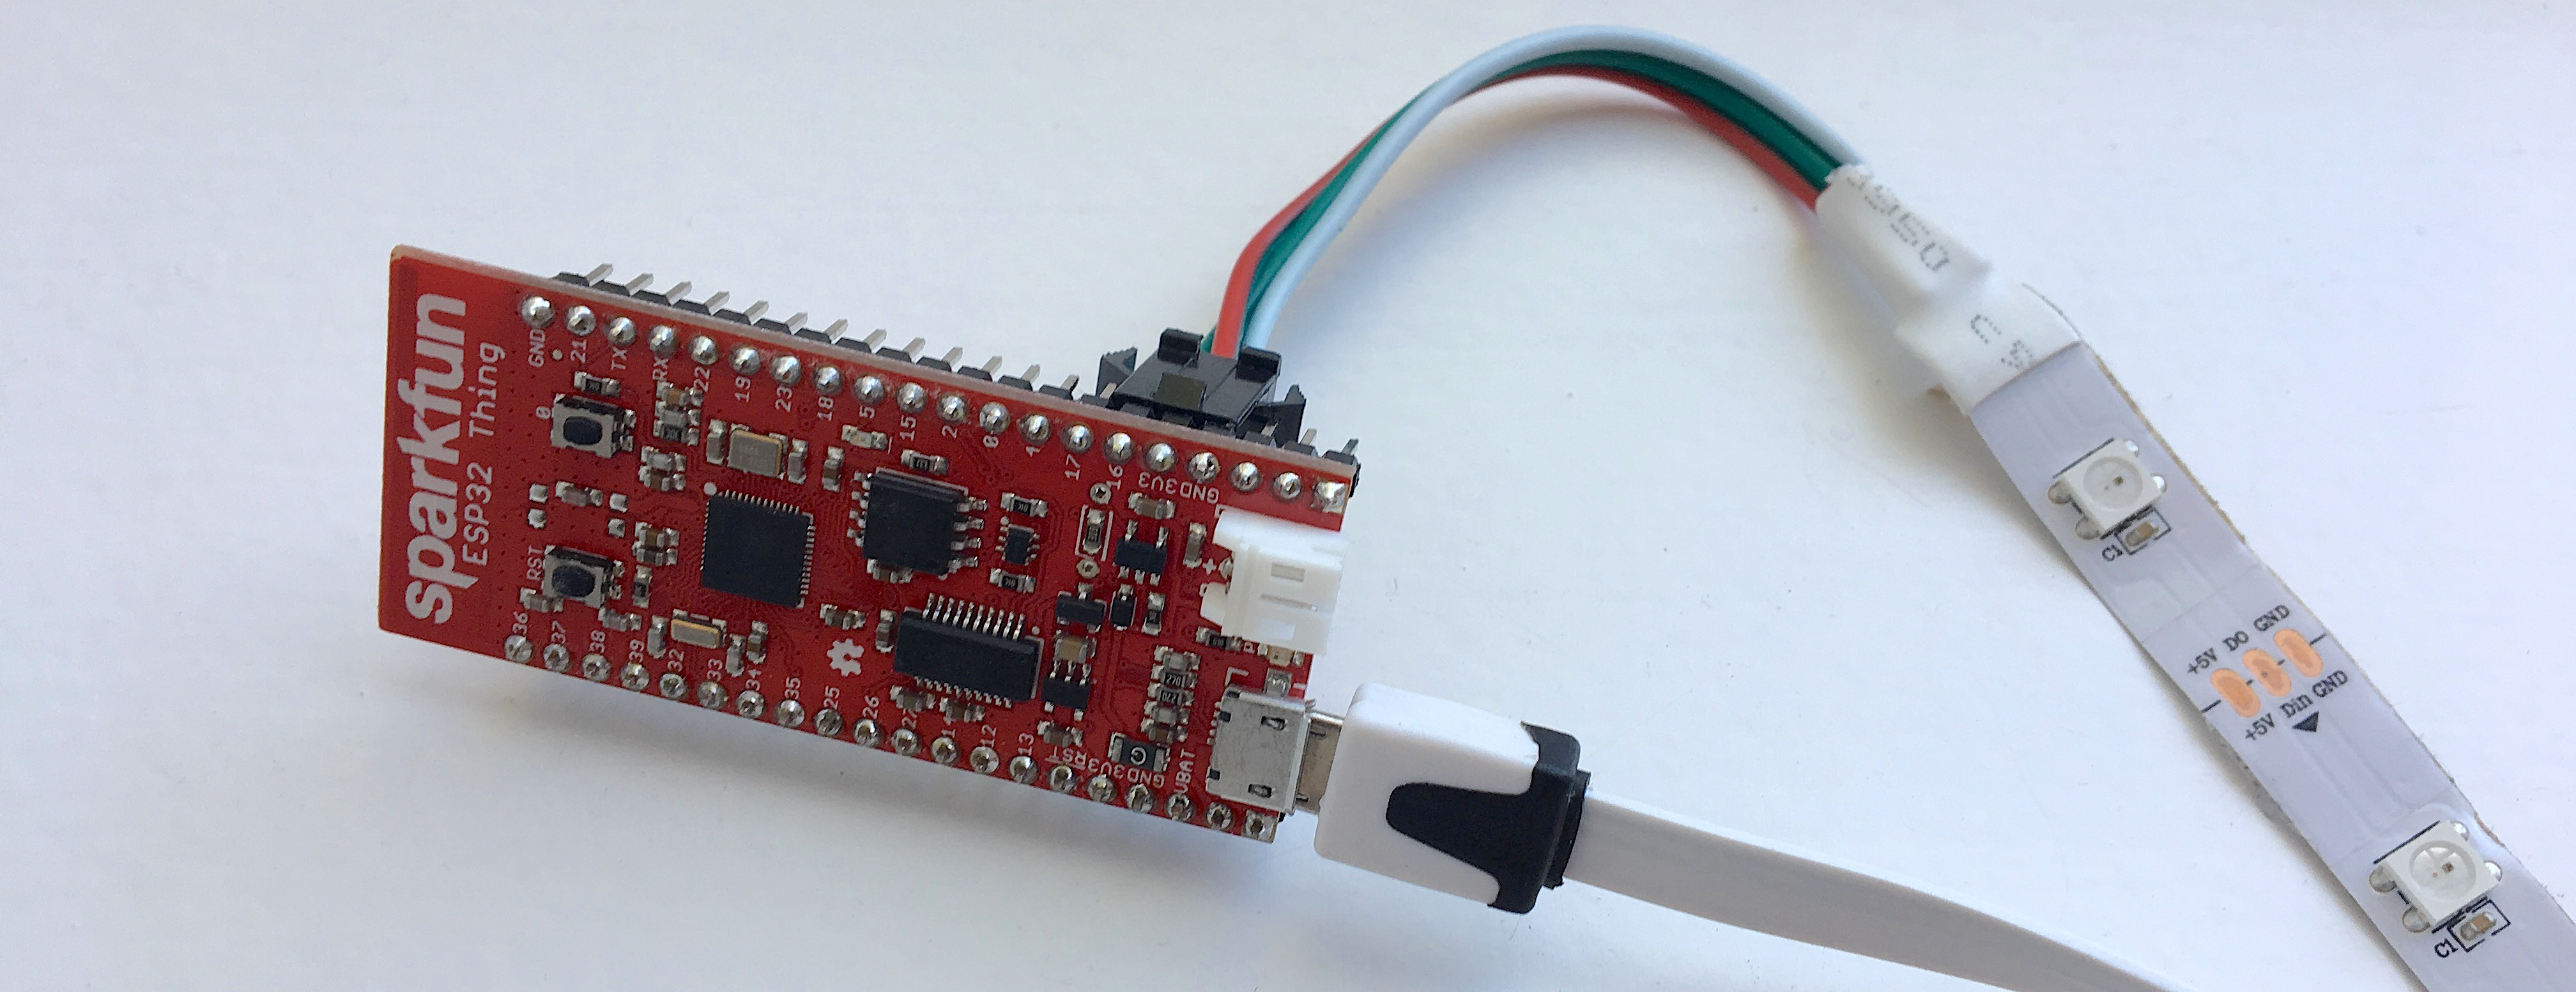
\includegraphics[width=0.9\textwidth]{illustrations/ledstrip-connection}
\end{center}

Forbindelserne er:
\begin{center}
\begin{tabular}{llll}
  \textbf{Ledningsfarve} & \textbf{Type} & \textbf{ESP32 pin} & \textbf{LED-strip} \\
  \hline
 Hvid & Jord & GND & GND \\
 Rød & 3.3V & 3V3 & 5VDC \\
 Grøn & Kontrolsignal & Pin 16 & DIN
\end{tabular}
\end{center}
\end{exercisebox}

\begin{exercisebox}[adjusted title=Første MicroPython program]
Åbn Mu-editoren. Opret en fil ``ledstrip\_demo.py'' med dette indhold:
\begin{python}
import machine
import neopixel

# 30 LED'er tilsluttet pin 16
ledstrip = neopixel.NeoPixel(machine.Pin(16), 30)

# Indstil LED'ernes farver
ledstrip[0] = (255, 0, 0)
ledstrip[9] = (0, 0, 255)

# Opdater LED'erne ved at kalde ledstrip.write()
ledstrip.write()
\end{python}

\tcbsubtitle{Afprøv programmet}
\begin{itemize}
\item Tryk på Run-knappen i Mu for at køre programmet på Microcontrolleren.
\item Tjek, at den første diode lyser rødt (diode 0) og den tiende lyser blåt (diode 9).
\end{itemize}

\tcbsubtitle{Opgaver}
\begin{itemize}
\item Udvid programmet, så hver anden diode farves rød og hver anden farves blå for de første 10 dioder.
\item \textit{Gør koden pænere}: Opret variable til farverne (\ttpy{blue = (0, 0, 255)}, osv.).
\end{itemize}
\end{exercisebox}
\newpage
\begin{exercisebox}[adjusted title=Animationer]
For at lave animationer skal vi bruge funktionen \ttpy{sleep_ms} fra
biblioteket \ttpy{time}.

\begin{python}
import machine
import neopixel
import time

red = (255, 0, 0)
blue = (0, 0, 255)

ledstrip = neopixel.NeoPixel(machine.Pin(16), 30)

# Tænd den første diode
ledstrip[0] = red
ledstrip.write()

# Vent 200 millisekunder
time.sleep_ms(200)

# Tænd den næste diode
ledstrip[1] = blue
ledstrip.write()
time.sleep_ms(200)

# Fortsæt selv ...
\end{python}

\tcbsubtitle{Opgaver}
\begin{itemize}
\item Fortsæt mønsteret for de første 10 LED'er.
\item En LED slukkes ved at sætte den til (0, 0, 0). Sluk den forrige
  LED i hvert trin, så der kun er en LED tændt ad gangen.
%\item \textit{Gør koden pænere}: Lav en variabel til at styre hastigheden.
\end{itemize}
\end{exercisebox}

\begin{exercisebox}[adjusted title=Gør koden pænere: Variable og Funktioner]
\begin{itemize}
\item Lav en variabel til at styre hastigheden (delayet).
\item Skriv en funktion \ttpy{fill(leds, color)}, der tænder alle LED'nerne i
  den givne farve (tænd kun de 10 første - vi gør den smartere senere).
\item Skriv en funktion \ttpy{clear(leds)}, der slukker alle LED'erne (kun de 10 første).
\item Skriv kode der afprøver \ttpy{fill()} og \ttpy{clear()}
  funktionerne. Kør koden og tjek at de virker som forventet.
\end{itemize}
\end{exercisebox}
% Lad os få optimeret den gentagne kode væk ved at bruge funktioner.

% \noindent
% Opret en funktion \ttpy{fill} der tænder LED'erne i en given farve:
% \begin{python}
% def fill(leds, color):
%     leds[0] = color
%     leds[1] = color
%     leds[2] = color
%     leds[3] = color
%     leds[4] = color
%     leds[5] = color
%     leds[6] = color
%     leds[7] = color
%     leds[8] = color
%     leds[9] = color
%     leds.write()
% \end{python}

% \noindent
% Funktionen kaldes sådan:
% \begin{python}
% fill(ledstrip, green)
% \end{python}

% \noindent
% Opgaver:
% \begin{itemize}
% \item Skriv en funktion \ttpy{clear(leds)} der slukker alle dioderne.
% \item Brug funktionen \ttpy{fill(leds, color)} i \ttpy{weather.py} til
%   at styre LED-strippen.
% \end{itemize}


\begin{exercisebox}[adjusted title=Mini-projekt]
  Lav en regnbue, en istap, animation af ild, eller
  noget kunstnerisk i selv finder på. Brug max 10 minutter. Her er
  nogle flere farver:

  \hfill \\
  \begin{minipage}{0.45\linewidth}
    \begin{tabular}{ll}
    \textbf{Rød} & \lstinline[style=mypython]$(255, 0, 0)$ \\
    \textbf{Grøn} & \lstinline[style=mypython]$(0, 255, 0)$ \\
    \textbf{Blå} & \lstinline[style=mypython]$(0, 0, 255)$ \\
    \textbf{Hvid} & \lstinline[style=mypython]$(255, 255, 255)$ \\
    \end{tabular}
  \end{minipage}
  \begin{minipage}{0.45\linewidth}
    \begin{tabular}{ll}
    \textbf{Slukket} & \lstinline[style=mypython]$(0, 0, 0)$ \\
    \textbf{Gul} & \lstinline[style=mypython]$(255, 255, 0)$ \\
   \textbf{Lilla} & \lstinline[style=mypython]$(127, 0, 255)$ \\
    \textbf{Tyrkis} & \lstinline[style=mypython]$(0, 255, 255)$ \\
    \end{tabular}
  \end{minipage}
\end{exercisebox}

% \chapter{Fading}
% Ud over at man kan skifte hvilke af af dioderne er tændt med hvilken
% farve, kan lysintensiteten også ændres, så man kan lave fading-effekter.

% \noindent
% \begin{minipage}{0.50\linewidth}
% \begin{lstlisting}[style=mypython, escapechar=@]
% def fill(np, color):
%     np[0] = color
%     np[1] = color
%     np[2] = color
%     np[3] = color
%     np[4] = color
%     np[5] = color
%     np[6] = color
%     np[7] = color
%     np.write()
% @~@
% @~@
% \end{lstlisting}
% \vspace{2em}
% \end{minipage}
  % \quad
% \begin{minipage}{0.45\linewidth}
% \begin{python}
% def fadeOutRed(np, delay):
%     fill(np, (64, 0, 0))
%     time.sleep_ms(delay)
%     fill(np, (48, 0, 0))
%     time.sleep_ms(delay)
%     fill(np, (32, 0, 0))
%     time.sleep_ms(delay)
%     fill(np, (16, 0, 0))
%     time.sleep_ms(delay)
%     fill(np, (0, 0, 0))
%     time.sleep_ms(delay)

% np = neopixel.NeoPixel(machine.Pin(19), 8)
% fadeOutRed(np, 1000)
% \end{python}
% \end{minipage}

\newpage
\stepcounter{handout}
\renewcommand{\Title}{\Ark Internetforbindelse}
\begin{exercisebox}[adjusted title=Overfør wifi-modul]
Før vi kan logge på Wifi, skal vi bruge et lille modul, der gør det lettere.
\begin{itemize}
\item Download filen ``\ttpy{wifi.py}'' fra kursussiden på
  Absalon og gem den i mappen ``mu\_code'' på din computer
\item Tryk på ``Files'' i Mu og træk filen ``\ttpy{wifi.py}'' fra højre side til venstre side for at
    overføre den til microcontrolleren
\end{itemize}
\end{exercisebox}

\begin{exercisebox}[adjusted title=Forbind til WiFi]
\vspace{-2mm}
Opret en ny fil med følgende indhold og gem som ``\ttpy{wifi_test.py}'':
\begin{python}
import wifi
wifi.connect("FemTech.dk2", "0F76FMYHB0Q")
\end{python}

\noindent
Når du kører filen, burde den skrive følgende (og et par andre
linjer):
\begin{lstlisting}
Connecting to WiFi network...
Successfully connected to "FemTech.dk2".
\end{lstlisting}
\vspace{-4mm}
\end{exercisebox}
% \noindent
% Hvis du kører den flere gange skriver den:
% \begin{lstlisting}
% Already connected.
% \end{lstlisting}

\begin{exercisebox}[adjusted title=Hent vejrdata fra OpenWeatherMap]
\vspace{-2mm}
Vi har forberedt et MicroPython projekt, der henter vejrdata fra OpenWeatherMap.org:
\begin{itemize}
\item Hent ``\ttpy{weather.py}'' fra kursussiden på Absalon
\item Åbn den i Mu-editoren og prøv at køre koden
\end{itemize}

% \noindent
% Tilføj de her linjer kode:
% \begin{python}
% openWeatherMap_APIKey = "0954b75734e22fc17947b9923359ee7b"

% def getWeatherData(city):
%     requestUrl = ("http://api.openweathermap.org/data/2.5/weather?q="
%                    + city + "&units=metric&appid=" + openWeatherMap_APIKey)
%     response = urequests.get(requestUrl)
%     return response.json()
    
% # Hent vejrdata
% weatherData = getWeatherData("Copenhagen")

% # Vis vejrdata
% print(weatherData)
% \end{python}

% \vspace{2mm}
% \noindent
Nu burde der i konsol-vinduet blive vist noget i stil med:
{\tiny
\begin{python}
{'timezone': 7200, 'cod': 200, 'dt': 1561470780, 'base': 'stations',
  'weather': [{'id': 804, 'icon': '04d', 'main': 'Clouds',
               'description': 'overcast clouds'}],
  'sys': {'message': 0.0076, 'country': 'DK',  'sunrise': 1561429582,
          'sunset': 1561492681, 'id': 1575, 'type': 1},
  'name': 'Copenhagen', 'clouds': {'all': 100}, 'coord': {'lon': 12.57, 'lat': 55.69},
  'visibility': 10000, 'wind': {'speed': 5.1, 'deg': 150}, 'id': 2618425,
  'main': {'pressure': 1023, 'humidity': 64, 'temp_min': 23.89,
           'temp_max': 28.33, 'temp': 26.27}}
Temperatur i Koebenhavn: 26.27
\end{python}
}
\vspace{-4mm}
\end{exercisebox}
\noindent
%Forklaring følger på næste side.
% \chapter{Hent vejrdata fra OpenWeatherMap}
%   Tilføj de her linjer kode:
% \begin{python}
% def get_carbon_intensity():
%     requestUrl = "http://api.electricitymap.org/v3/carbon-intensity/latest?zone=DK-DK2"
%     headers = {'auth-token': "G3EnPfUtfg2ng4PyZ2CRwh"}
%     response = urequests.get(requestUrl, headers=headers)
%     dataObject = response.json()
%     return dataObject["carbonIntensity"]

% # Hent CO2-data
% co2level = get_carbon_intensity()

% # Vis CO2-data i REPL
% print(co2level)
% \end{python}


% \newpage

\begin{exercisebox}[adjusted title=Aflæs enkeltværdier]
\vspace{-2mm}
Ovenstående udskrift kan læses som: ``'timezone' har værdien 7200,
'cod' har værdien 200, 'dt' har værdien 1561470780'' og så
videre. Længere nede kan man se, at 'wind' har værdien \ttpy|{'speed':  5.1, 'deg' : 150}|,
det betyder, at 'wind' indeholder to navngivne værdier ('speed' og 'deg')

\vspace{1mm}
\noindent
I Python gør man som følger for at aflæse de enkelte værdier:
\begin{python}
# Aflæs sigtbarhed (i meter)
visibility = weather_data["visibility"]
# Aflæs temperatur til variabel (grader celcius)
temperature = weather_data["main"]["temp"]
# Aflæs vindhastighed (i meter pr. sekund)
windspeed = weather_data["wind"]["speed"]\end{python}
\vspace{-4mm}
\end{exercisebox}
\newpage

\begin{exercisebox}[adjusted title=Vælg mellem farver]

Tilføj LED-strip initialisering øverst i ``\ttpy{weather.py}'' (efter \ttpy{import}'s):
\begin{python}
ledstrip = neopixel.NeoPixel(machine.Pin(16), 30)

green = (0, 255, 0)
blue = (0, 0, 255)
\end{python}

\noindent
Kopier dine \ttpy{fill()} og \ttpy{clear()} funktioner fra tidligere
ind i ``\ttpy{weather.py}''.

\vspace{2mm}
\noindent
Tilføj derefter følgende linjer kode nederst i ``\ttpy{weather.py}'':
\begin{python}
# Funktionen tempToColor konverterer en temperatur i grader celcius
# til en (r,g,b)-farve værdi
def tempToColor(temp):
    # Grøn hvis 15 grader eller højere
    # Blå hvis lavere end 15 grader
    if temp >= 15:
        return green
    else:
        return blue 

color = tempToColor(temperature)
fill(ledstrip, color)
\end{python}
\vspace{-2mm}
\tcbsubtitle{Opgaver}

\begin{itemize}
\item Ændr ``\ttpy{tempToColor}'' så LED'erne farves røde, når
  temperaturen er over 35 \textdegree C
\item Ændr ``\ttpy{tempToColor}'' så LED'erne farves gule, når temperaturen er 25-35\textdegree C
\item Ændr ``\ttpy{tempToColor}'' så LED'erne farves hvide, når temperaturen er under 0\textdegree C
\end{itemize}
\end{exercisebox}
\begin{exercisebox}[adjusted title=Gentag uendeligt]
Næste skridt er at sørge for, at vores vejr-melding bliver ved
med at opdatere sig.

I MicroPython er der ikke en draw-funktion som i Processing, men vi
kan skrive tilsvarende selv. Hvis der er kode, vi vil have kørt igen
og igen kan man skrive ``\ttpy{while True:}'' og alle linjer der er
rykket ind med 4 mellemrum bagefter, vil så blive gentaget uendeligt
mange gange (eller ind til programmet stoppes).

\begin{lstlisting}[escapechar=@]
@\textbf{while} \textbf{True}@:
    @\textit{kommandoer der skal gentages}@
\end{lstlisting}

\noindent
Nu er opgaven at få jeres kode til minde om følgende
pseudokode\footnote{``Pseudo'' referer til at det er kode der
  \textit{minder om det rigtige, men ikke er fuldstændig lig det}. I kender allerede
  pseudo-præfikset fra ord som pseudonym eller pseudointellektuel.}:
\begin{lstlisting}[escapechar=@]
Gentag uendeligt:
    1. Log på Wifi
    2. Hent vejr data
    3. Sluk alle dioder
    4. Vis vejrdata på lysdioder
    5. Log af Wifi
    6. Vent 2 minutter
\end{lstlisting}

\noindent
(Man logger af Wifi ved at skrive \ttpy{wifi.disconnect()})
\end{exercisebox}
\newpage
\stepcounter{handout}
\renewcommand{\Title}{\Ark Løkker}

\begin{exercisebox}[adjusted title=For-løkken]
Der er noget utilfredsstillende ved, at vi er blevet nødt til at
skrive så mange linjer, der minder om hinanden:
\begin{python}
leds[0] = color
leds[1] = color
leds[2] = color
leds[3] = color
...
\end{python}
Og hvordan skulle vi programmere, hvis vi ville have LED-strippen til at lyse med 17
LED'er, når temperaturen er 17 grader celcius?

 I stedet for at gentage samme kommando igen og igen kan vi bruge
\textit{løkker} (eng. loops), de gør det nemt at gentage de samme
kommandoer mange gange. Vi har allerede set et eksempel på en løkke:
\ttpy{while}-løkken. Nu skal vi lære om for-løkken.

  
Opret en ny fil \ttpy{loops.py}:
\begin{python}
  import machine
  import neopixel
  import time

  ledstrip = neopixel.NeoPixel(machine.Pin(16), 30)
  purple = (127, 0, 255)

  for i in range(30):
      ledstrip[i] = purple
      ledstrip.write()
      time.sleep_ms(100)
\end{python}

\tcbsubtitle{Opgaver}
\begin{enumerate}
\item Prøv at ændre \ttpy{range(30)} til \ttpy{range(17)} eller \ttpy{range(3)}
\item Prøv at tilføje linjen \ttpy{print(i)} inde i løkken for at se,
  hvordan variablen \ttpy{i} ændrer sig
\item Skriv en løkke der slukker alle LED'er (øjeblikkeligt - intet sleep)
\item Omskriv funktionen \ttpy{fill(leds, color)}, så den slukker alle LED'er (ikke bare de 10 første)
\item Skriv en ny funktion \ttpy{fillN(leds, color, n)}, der tænder de
  \ttpy{n} første LED'er
\item Skriv en løkke, der tænder hver anden LED (dem med lige
  index)\footnote{Tip: En løsning kan være kun at tælle til 15, men
    lave en lille beregning på indexet. En anden løsning bruger
    modulus (se ark \#4 fra uge 1).}
\item Skriv en løkke, der tænder LED'erne én ad gangen, men starter fra
  den sidste (29) og slutter med den første (0) - søg gerne hjælp online.
\end{enumerate}
\end{exercisebox}
\newpage
\hfill

\newpage
\stepcounter{handout}
\renewcommand{\Title}{\Ark Keypad}
\begin{exercisebox}[adjusted title=Tilslut keypad]
  Tilslut et Keypad som vist på billedet:
  
\noindent
\begin{minipage}{0.65\linewidth}
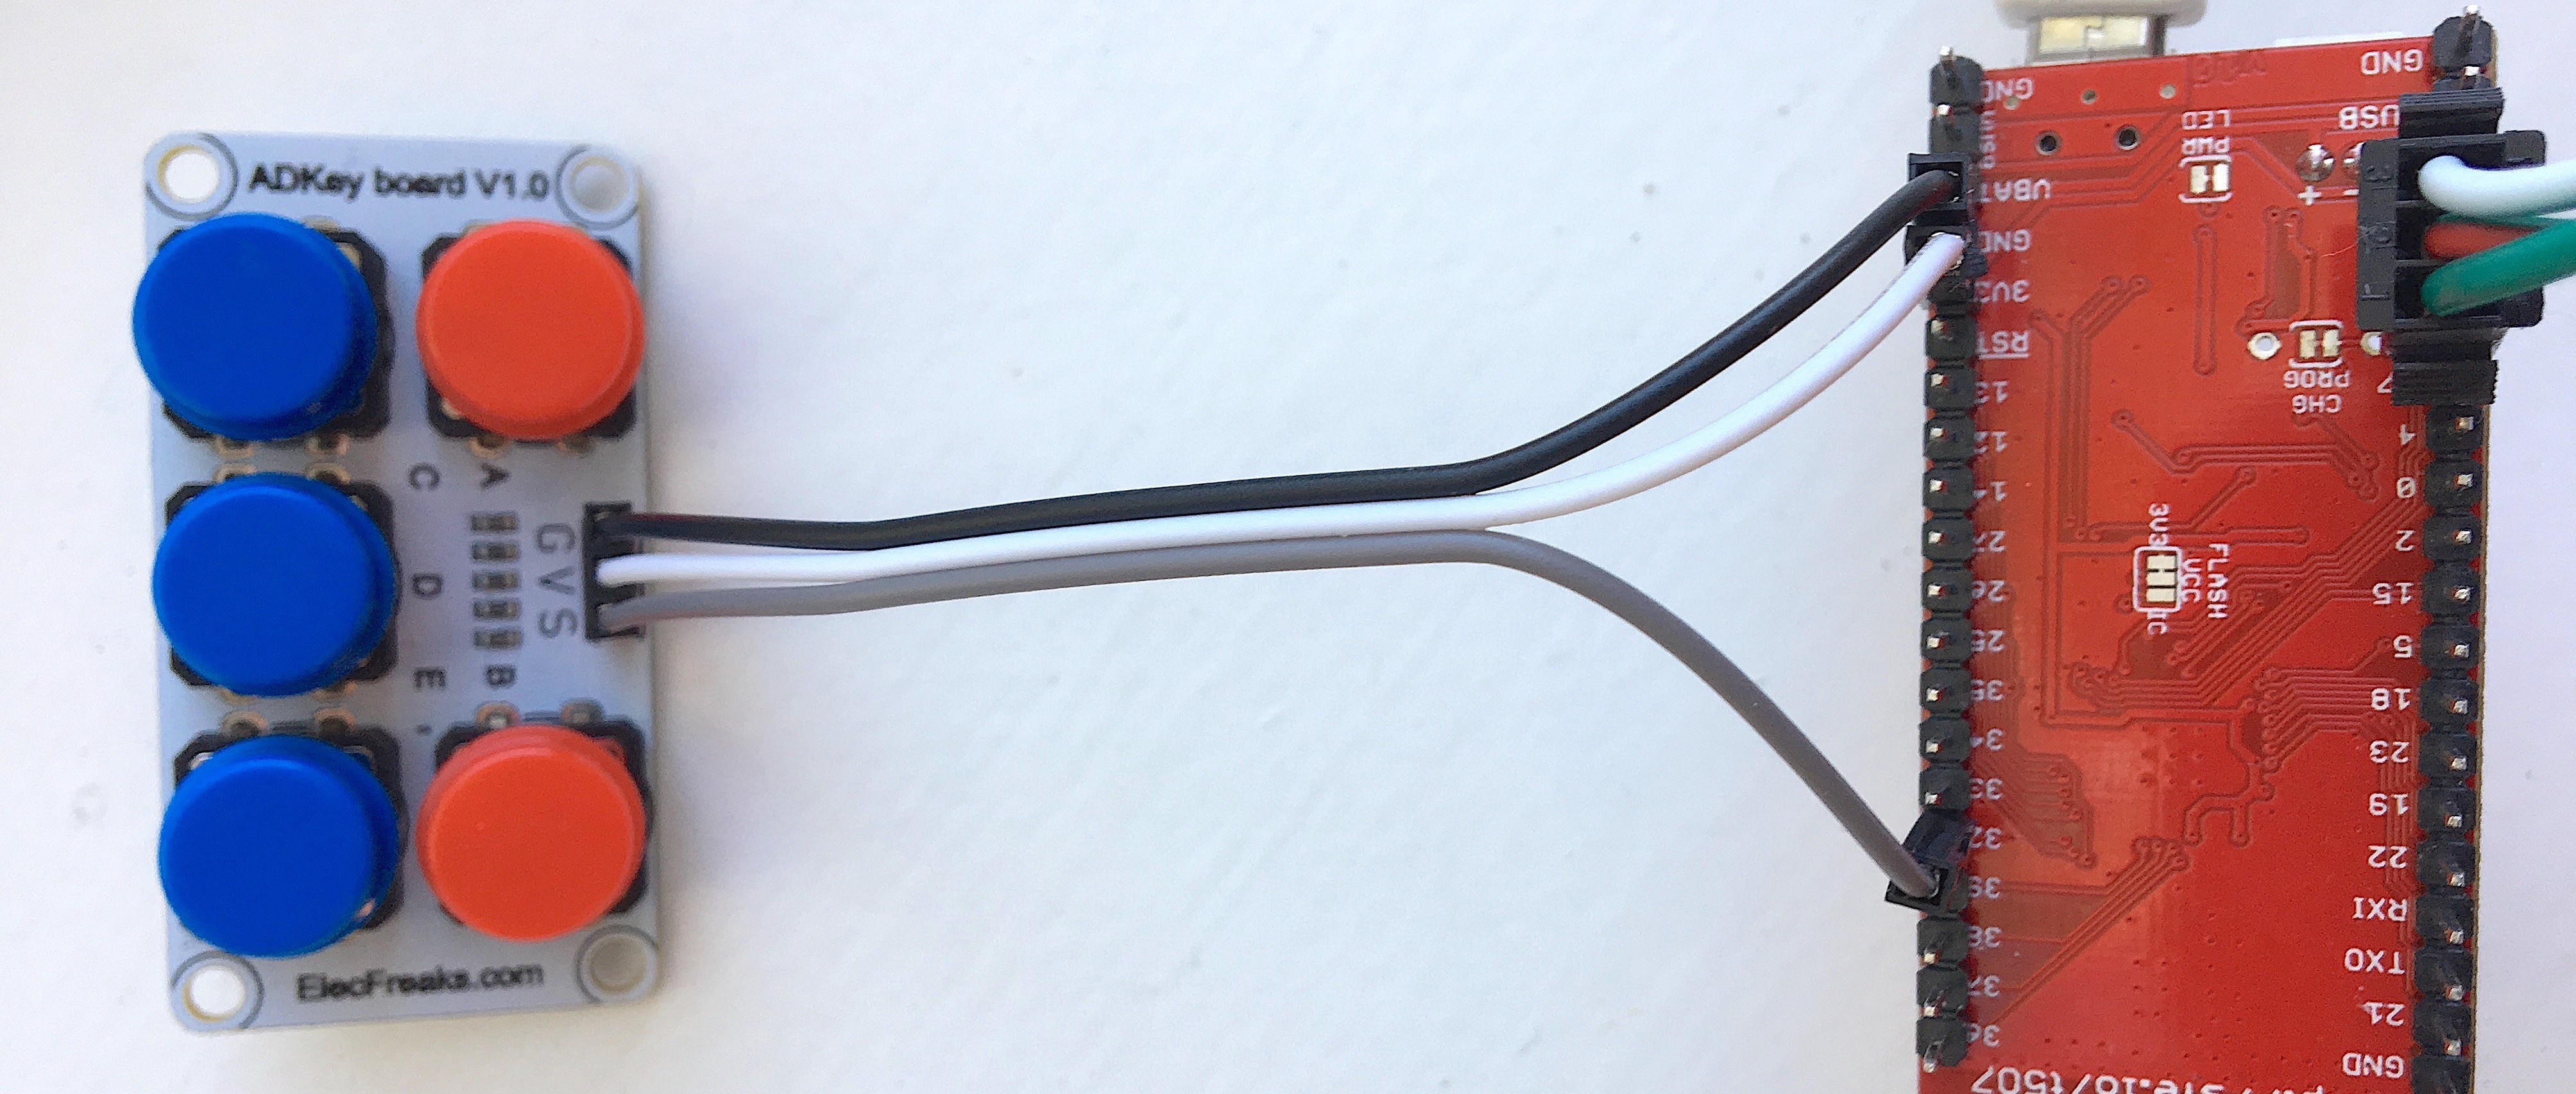
\includegraphics[width=\textwidth]{illustrations/keypad-connection-cropped}
\end{minipage}
\begin{minipage}{0.20\linewidth}
\noindent
\begin{tabular}{lll}
  Type & ESP32 & Keypad \\
  \hline
 Jord & GND & G \\
 3.3V & 3V3 & V \\
 Signal & Pin 32 & S
\end{tabular}

\end{minipage}
\tcbsubtitle{Hent og overfør TinkerLib}
\begin{itemize}
\item Hent filen ``tinkerlib.py'' fra Absalon
\item Overfør den til microcontrolleren på samme måde som med \ttpy{wifi.py}
\end{itemize}
\end{exercisebox}

\begin{exercisebox}[adjusted title=Programmering af keypad]
Her er et eksempel, på hvordan keypaddet bruges:
\begin{python}
import machine
import tinkerlib

def keypadButtonDown(key):
    print(key)

pin32 = machine.Pin(32, mode=machine.Pin.IN)
keypad = tinkerlib.ADKeypad(pin32, button_down=keypadButtonDown)
\end{python}

\noindent
Prøv at køre programmet og tryk på knapperne.

\vspace{2mm}
\noindent
Funktionen \ttpy{keypadButtonDown} bliver kaldt hver gang, der bliver
trykket på en af knapperne, lidt ligesom \ttpy{keyPressed} i
Processing. Argumentet key er et tal mellem 0 og 4, afhængigt af
hvilken knap der blev trykket på.
\end{exercisebox}

\begin{exercisebox}[adjusted title=Simpel nedtælling]
Indtast følgende i slutningen af samme fil og kopier funktionerne
``\ttpy{clear}'' og ``\ttpy{fillN}'', som I skrev i filen ``loops.py''. Husk også at importere \ttpy{neopixel} og \ttpy{time} modulerne.

\begin{python}
timeleft = 30000
blue = (0, 0, 255)
ledstrip = neopixel.NeoPixel(machine.Pin(16), 30)

while True:
    clear(ledstrip)
    fillN(ledstrip, blue, timeleft/1000)
    timeleft = timeleft - 10
    time.sleep_ms(10)
\end{python}

\noindent
I skal nu ændre ovenstående kode til at bruge keypaddet til at styre
``timeleft''. Én af knapperne skal lægge 1000 til timeleft, en anden
skal trække 1000 fra.
\end{exercisebox}

\begin{exercisebox}[adjusted title=Æggeur]
Vi skal nu have kodet vores lille nedtællingsur om til at blive et
funktionelt æggeur (eller pair-programming ur).

Før vi går i gang med at kode en løsning, skal vi planlægge, hvordan
det skal virke. I denne omgang har vi på forhånd bestemt hvordan, og
uret skal derfor virke efter følgende tilstandsdiagram:

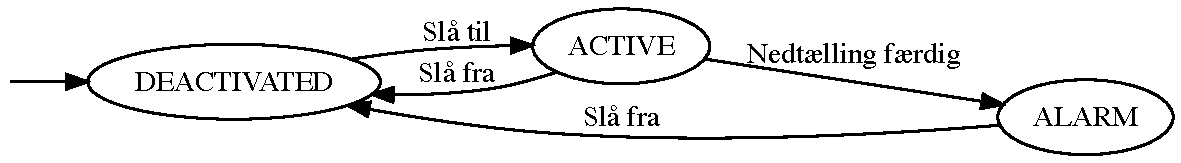
\includegraphics[width=1.0\textwidth]{graphviz/alarm}

\noindent
Opret en global variabel \ttpy{alarm_state} og sæt den til ``DEACTIVATED''.


\tcbsubtitle{Visning (View)}
Vi kan opdele ændringerne i det, der har med visning at gøre, og det
der har med styring at gøre. Her først de ændringer I skal lave
ifht. visning:

\begin{enumerate}
\item Når tilstanden er DEACTIVATED vises minutter tilbage i rød farve
\item Når tilstand er ACTIVE vises minutter tilbage i blå farve
\item Når tilstanden er ALARM tændes alle 30 LED'er i grøn farve
\end{enumerate}

\vspace{-3mm}
\tcbsubtitle{Styring (Control)}
Nu skal I ændre, hvordan styringen skal fungere jvf. tilstandsdiagrammet.

Først skal i ændre i \ttpy{while}-løkken:
\begin{enumerate}
\setcounter{enumi}{3}
\item \ttpy{timeleft} skal kun tælle ned, når tilstanden er ACTIVE.
\item Hvis tiden er gået (timeleft <= 0) og tilstanden er ACTIVE, så skal der skiftes tilstand til ALARM.
\end{enumerate}

\noindent
Derefter skal I ændre i \ttpy{keypadButtonDown}:
\begin{enumerate}
    \setcounter{enumi}{5}
\item Hvis der bliver trykket på ``sæt alarm'' knappen og tilstanden er DEACTIVATED, skiftes tilstand til ACTIVE.
\item Hvis der bliver trykket på ``sæt alarm'' knappen og tilstanden er ACTIVE eller ALARM, skiftes tilstand til DEACTIVATED.
  \\
  Samtidig sættes timeleft tilbage til 7 minutter (420000ms).

\end{enumerate}

\tcbsubtitle{Tæl i minutter frem for timer}
Lad os ændre uret til at tælle minutter frem for sekunder:
\begin{enumerate}
\setcounter{enumi}{7}
\item Sæt \ttpy{timeleft} til 7 minutter (420000ms) når programmet starter
\item Hvis der trykkes på ``forøg'', lægges der et minut (60000ms) til \ttpy{timeleft}
\item Hvis der trykkes på ``reducer'', trækkes der et minut (60000ms) fra \ttpy{timeleft}
\item Ved visning af resterende tid divideres \ttpy{timeleft} med yderligere 60.
\end{enumerate}
\end{exercisebox}

\end{document}
